\documentclass[10pt]{amsart}
\usepackage{amsmath,amsthm,amssymb,amsfonts,enumerate,mymath,mathtools,tikz}
\usetikzlibrary{shapes}

\openup 5pt
\author{Blake Farman\\University of South Carolina}
\title{Math 702:\\Homework 05}
\date{March 1, 2013}
\pdfpagewidth 8.5in
\pdfpageheight 11in
\usepackage[margin=1in]{geometry}

\begin{document}
\maketitle

\providecommand{\p}{\mathfrak{p}}
\providecommand{\m}{\mathfrak{m}}

\newtheorem{thm}{}
\newtheorem{lem}{Lemma}

\newcommand{\End}[2]{\operatorname{End}_{#1}\left(#2\right)}
\newcommand{\Hom}[2]{\operatorname{Hom}_{#1}\left(#2\right)}

\begin{thm}
  Recall that the splitting field of $x^4 - 2$ is $K = \Q(\sqrt[4]{2}, i)$, and that $[K : \Q] = 8$.
  \begin{enumerate}[(a)]
  \item
    Define $\sigma$ on $K$ by $\sigma(\sqrt[4]{2}) = i\sqrt[4]{2}, \sigma(i) = i$;
    define $\tau$ on $K$ by $\tau(\sqrt[4]{2}) = \sqrt[4]{2}, \tau(i) = -i$.
    Confirm that $\sigma, \tau \in \Gal{K/\Q}$, and list all the elements of $\Gal{K/\Q}$.
    Can you identify (up to isomorphism) $\Gal{K/\Q}$ as a familiar group?
  \item
    Determine the fixed field of $\left<\sigma^2\tau\right>$.
  \item
    What is $\Gal{K/\Q(\sqrt{2}, i)}$?
  \item
    Draw the subgroup and subfield diagrams for $\Gal{K/\Q}$ and $K/\Q$.
    Label all degrees.
  \end{enumerate}
  
  \begin{proof}
    \begin{enumerate}[(a)]
    \item
      It is clear that both $\sigma$ and $\tau$ fix $\Q$ and hence are not trivial.
      To see that they are automorphisms, observe that for every $a, b, c \in \Q$
      $$a + ib + c\sqrt[4]{2} \xmapsto{\sigma} a + ib + ic\sqrt[4]{2} \in K\ \text{and}\ a + ib + c\sqrt[4]{2} \xmapsto{\tau} a - ib + c\sqrt[4]{2} \in K.$$
      Therefore $\sigma, \tau \in \Gal{K/\Q}$.
      
      The Galois group is
      $$\Gal{K/\Q} = \left< \sigma, \tau \;\middle\vert\; \sigma^4 = \tau^2 = 1,\, \sigma\tau = \tau\sigma^3 \right>$$
      and the isomorphism type is $D_8$.
      Explicitly, the maps other than 1, $\sigma$, and $\tau$ are
      $$\begin{array}{ccc}
      \sigma^2 \colon \left\{
      \begin{array}{l}
        \sqrt[4]{2} \mapsto -\sqrt[4]{2}\\
        i \mapsto i
      \end{array}
      \right.&
      \sigma^3 \colon \left\{
      \begin{array}{l}
        \sqrt[4]{2} \mapsto -i\sqrt[4]{2}\\
        i \mapsto i\\
      \end{array}
      \right.&
      \tau\sigma \colon
      \left\{
      \begin{array}{l}
        \sqrt[4]{2} \mapsto -i\sqrt[4]{2}\\
        i \mapsto -i\\
      \end{array}
      \right.\\
      \tau\sigma^2 \colon \left\{
      \begin{array}{l}
        \sqrt[4]{2} \mapsto -\sqrt[4]{2}\\
        i \mapsto -i\\
      \end{array}
      \right.
      &
      \tau\sigma^3 \colon 
      \left\{
      \begin{array}{l}
        \sqrt[4]{2} \mapsto i\sqrt[4]{2}\\
        i \mapsto -i\\
      \end{array}
      \right.
      \end{array}.$$
    \item
      First observe that $\sigma^2\tau = \tau\sigma^2$.
      Since $[\Gal{K/\Q} : \left<\tau\sigma^2\right>] = 4$, the fixed field has degree 4 over $\Q$.
      Then $\tau\sigma^2(i\sqrt[4]{2}) = \tau(i(-\sqrt[4]{2})) = -i(-\sqrt[4]{2}) = i\sqrt[4]{2}$ shows that $K^{\left<\tau\sigma^2\right>} = \Q(i\sqrt[4]{2})$.
    \item
      Since $\Q(i,\sqrt{2}) = \Q(\sqrt{2})(i)$, it has degree 4 over $\Q$ and thus $\Gal{K/\Q(\sqrt{2}, i)}$ must be a group of order two.
      It is clear that any morphism involving $\tau$ will not fix $i$, so the only choice is $\left<\sigma^2\right>$.
      Indeed, $\sigma^2(i) = i$ and 
      $$\sigma^2(\sqrt{2}) = \sigma^2(\sqrt[4]{2}^2) = (\sigma^2(\sqrt[4]{2}))^2 = (- \sqrt[4]{2})^2 = \sqrt{2}.$$
    \item
      The subfield and subgroup lattices are given below, with the subgroup lattice inverted to be in correspondence with the lattice of subfields.
      \begin{center}
        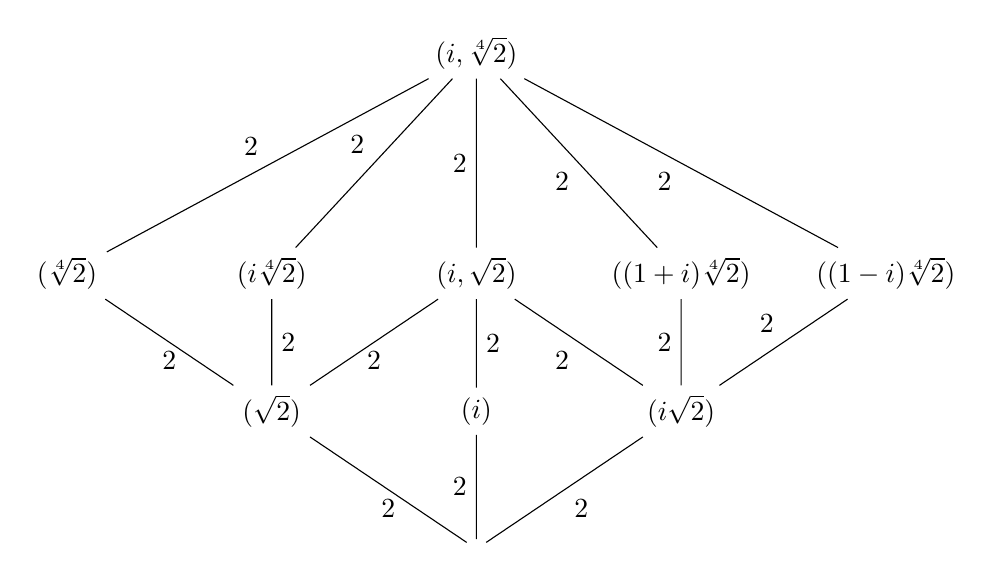
\begin{tikzpicture}[auto, xscale=.65, yscale=.35]
          \node(octic) at (8,23){$\Q(i, \sqrt[4]{2})$};
          \node(quart1) at (0,15){$\Q(\sqrt[4]{2})$};
          \node(quart2) at (4,15){$\Q(i\sqrt[4]{2})$};
          \node(quart3) at (8,15){$\Q(i, \sqrt{2})$};
          \node(quart4) at (12,15){$\Q((1 + i)\sqrt[4]{2})$};
          \node(quart5) at (16,15){$\Q((1 - i)\sqrt[4]{2})$};
          \node(quad1) at (4,10){$\Q(\sqrt{2})$};
          \node(quad2) at (8,10){$\Q(i)$};
          \node(quad3) at (12,10){$\Q(i\sqrt{2})$};
          \node(q) at (8,5){$\Q$};
          \draw (quad1) to node [below] {2} (q);
          \draw (quad2) to node [swap] {2} (q);
          \draw (quad3) to node {2} (q);
          \draw (quad1) to node [below] {2} (quart1);
          \draw (quad1) to node [swap] {2} (quart2);
          \draw (quad1) to node [below] {2} (quart3);
          \draw (quad2) to node [swap] {2} (quart3);
          \draw (quad3) to node {2} (quart3);
          \draw (quad3) to node {2} (quart4);
          \draw (quad3) to node {2} (quart5);
          \draw (quart1) to node {2} (octic);
          \draw (quart2) to node {2} (octic);
          \draw (quart3) to node {2} (octic);
          \draw (quart4) to node {2} (octic);
          \draw (quart5) to node {2} (octic);
        \end{tikzpicture}
        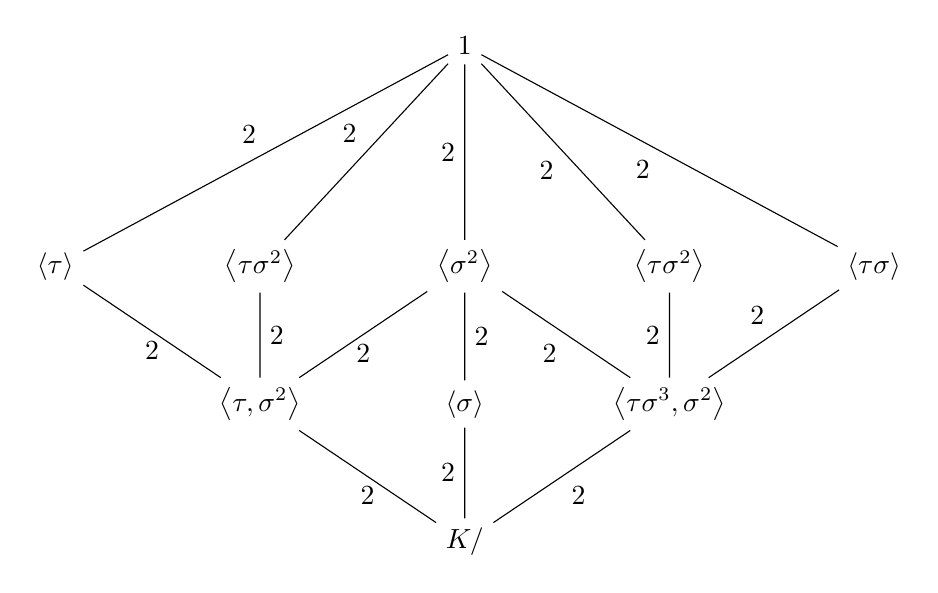
\begin{tikzpicture}[auto, xscale=.65, yscale=.35]
          \node(octic) at (8,23){$1$};
          \node(quart1) at (0,15){$\left<\tau\right>$};
          \node(quart2) at (4,15){$\left<\tau\sigma^2\right>$};
          \node(quart3) at (8,15){$\left<\sigma^2\right>$};
          \node(quart4) at (12,15){$\left<\tau\sigma^2\right>$};
          \node(quart5) at (16,15){$\left<\tau\sigma\right>$};
          \node(quad1) at (4,10){$\left<\tau,\sigma^2\right>$};
          \node(quad2) at (8,10){$\left<\sigma\right>$};
          \node(quad3) at (12,10){$\left<\tau\sigma^3, \sigma^2\right>$};
          \node(q) at (8,5){$\Gal{K/\Q}$};
          \draw (quad1) to node [below] {2} (q);
          \draw (quad2) to node [swap] {2} (q);
          \draw (quad3) to node {2} (q);
          \draw (quad1) to node [below] {2} (quart1);
          \draw (quad1) to node [swap] {2} (quart2);
          \draw (quad1) to node [below] {2} (quart3);
          \draw (quad2) to node [swap] {2} (quart3);
          \draw (quad3) to node {2} (quart3);
          \draw (quad3) to node {2} (quart4);
          \draw (quad3) to node {2} (quart5);
          \draw (quart1) to node {2} (octic);
          \draw (quart2) to node {2} (octic);
          \draw (quart3) to node {2} (octic);
          \draw (quart4) to node {2} (octic);
          \draw (quart5) to node {2} (octic);
        \end{tikzpicture}
      \end{center}
    \end{enumerate}
  \end{proof}
\end{thm}

\begin{thm}
  Let $p$ be prime, and let $n \geq 1$.
  Suppose that $K/F$ is Galois with $[K : F] = p^n$.
  Prove that there are Galois extensions of $F$ contained in $K$ with degrees $p$ and $p^{n-1}$.
  
  \begin{proof}
    By Homework 4 from last semester, $\Gal{K/F}$ has a normal subgroup of index $p$, $H$.
    By the Theorem from class and the Galois correspondence, $K^H/F$ is Galois and
    $$[K^H : F] = [\Gal{K/F} : H] = p.$$
    
    By the same exercise, $\Gal{K/F}$ has a non-trivial center, which is itself a $p$-group.
    Then by Cauchy's Theorem, there exists an element, $g$, of order $p$ contained in the center.
    Therefore the group $\left<g\right>$ is normal inside $\Gal{K/F}$, the field $K^{\left<g\right>}$ is Galois, and
    $$[K^{\left<g\right>} : F] = [\Gal{K/F} : \left<g\right>] = p^{n-1}.$$
  \end{proof}
\end{thm}

\begin{thm}
  \label{Ex3}
  This exercise determines $\Aut{\R/\Q}$
  \begin{enumerate}[(a)]
    \item
      Prove that any $\sigma \in \Aut{\R/\Q}$ takes squares to squares and takes positive reals to positive reals.
      Conclude that $a < b$ implies $\sigma a < \sigma b$ for every $a,b \in R$.
    \item
      Prove that $|a - b| < 1/m$ implies $|\sigma a - \sigma b|< 1/m$ for every positive integer $m$. 
      Conclude that $\sigma$ is a continuous map on $\R$.
    \item
      Prove that any continuous map on $\R$ which is the identity on $\Q$ is the identity map, hence $\Aut{\R/\Q} = 1$.
  \end{enumerate}

  \begin{proof}
    \begin{enumerate}[(a)]
    \item
      Let $x \in \R$ be given.
      Since $\sigma \in \Aut{\R/\Q}$, we have $\sigma(x^2) = (\sigma x)^2$.
      Hence $\sigma$ takes squares to squares.
      Then it follows that since each element $x$ of $\R^+$ can be written as a square, $\sigma x$ is also a square.
      Hence positive reals map to positive reals.
      Since $\sigma \in \Aut{\R/\Q}$, it must then be the case that no element of $\R^{\leq 0}$ maps into $\R^+$. 
      Then for $a < b$, we have $a - b < 0$ and thus $\sigma (a - b) = \sigma a - \sigma b < 0$.
      Therefore $\sigma a < \sigma b$.
    \item
      Let $0 < m \in \Z$ be given.
      Let $a,b \in \R$ be such that $\abs{a-b} < 1/m$.
      By assumption, $1/m$ is fixed under $\sigma$.
      It now follows from the result of part (a) that $-1/m < \sigma a - \sigma b < 1/m$.
      Letting $m$ tend to infinity, it follows from the density of $\Q$ in $\R$ that $\sigma$ is continuous on $\R$.
    \item
      Let $\sigma \in \Aut{\R/\Q}$ be given.
      Regard $\R$ as the set of equivalence classes of rational Cauchy sequences.
      For any element $x$ of $\R$, let $\{q_n\}_{n=1}^{\infty} \subseteq \Q$ be a representative.
      The result of part (b) implies that the sequence $\{\sigma q_n\}_{n=1}^{\infty} = \{q_n\}_{n=1}^{\infty}$ converges to $\sigma x$.
      Hence $\sigma x = x$ implies that $\sigma$ is the identity.
      Therefore, since the choice of $\sigma$ was arbitrary, $\Aut{\R/\Q} = 1$.
    \end{enumerate}
  \end{proof}
\end{thm}

\begin{thm}
  Let $k$ be a field, and let $k(t)$ be the field of rational functions in $t$ with coefficients in $k$.
  Prove that 
  $$\Aut{k(t)/k} = \left\{t \mapsto \frac{at + b}{ct + d} \;\middle\vert\; a, b, c, d \in k\ \text{and}\ ad - bc \neq 0\right\}.$$
  
  \begin{proof}
    Let $\sigma \in A = \left\{t \mapsto \frac{at + b}{ct + d} \;\middle\vert\; a, b, c, d \in k\ \text{and}\ ad - bc \neq 0\right\}$.
    Degree zero polynomials (i.e. elements of $k$) are clearly fixed by $\sigma$.
    Then for non-units $f,g \in k(t)$, we have 
    $$\sigma(f + g) = (f + g)(\frac{at + b}{ct + d}) = f(\frac{at + b}{ct + d}) + g(\frac{at + b}{ct + d}) = \sigma(f) + \sigma(g)$$
    and
    $$\sigma(fg) = (fg)\left(\frac{at + b}{ct + d}\right) = f\left(\frac{at + b}{ct + d}\right) g\left(\frac{at + b}{ct + d}\right) = \sigma(f)\sigma(g).$$
    Moreover, if $$\tau \colon t \mapsto \frac{dt - b}{ct + a}$$
    then
    $$\sigma\tau: t \xmapsto{\tau} \frac{dt - b}{-ct + a} \xmapsto{\sigma} \frac{d(at + b) - b(ct + d)}{-c(at + b) + a(ct + d)} = \frac{t(ad - bc) + (bd - bd)}{t(ac - ac) + (ad - bc)} = t$$
    and
    $$\tau\sigma: t \xmapsto{\sigma} \frac{at + b}{ct + d} \xmapsto{\tau} \frac{a(dt - b) + b(-ct + a)}{c(dt - b) + d(-ct + a)} = \frac{t(ad - bc) + (ab - ab)}{t(cd - cd) + (ad - bc)} = t.$$
    Hence $A \subseteq \Aut{k(t)/k}$.
    
    Conversely, let $\sigma \in \Aut{k(t)/k}$ be given.
    Since $\sigma$ fixes $k$, $\sigma \colon t \mapsto s$ for some $s \in k(t) \setminus k$.
    Regard $\sigma$ as an evalutation homomorphism (at $s$):
    \begin{align*}
      \sigma \colon k(t) & \rightarrow k(s)\\
      f(t) & \mapsto f(s).
    \end{align*}
    Since $\sigma \in \Aut{k(t)/k}$, it must be the case that $k(s) \cong k(t)$.
    By homework 5, exercise 2, we have that if we write $s = p(t)/q(t)$ with $p, q$ relatively prime, then 
    $$1 = [k(s) : k(t)] = \max\left\{\deg{p}, \deg{q}\right\}$$
    and so it follows that $\deg{p}, \deg{q} \leq 1$, but not both zero.
    That is 
    $$s = \frac{at + b}{ct + d}$$ 
    for some $a,b,c,d \in k$ with $a$ and $c$ not both zero.
    Moreover, if $ad - bc = 0$, then 
    $$s = \frac{at + b}{ct + d} = \frac{b}{d} \left(\frac{(a/b)t + 1}{(c/d)t + 1}\right) = \frac{b}{d} \left(\frac{(c/d)t + 1}{(c/d)t + 1}\right) = \frac{b}{d} \in k,$$
    contradicting the choice of $s$.
    Therefore $\Aut{k(t)/k} \subseteq A$, as desired.
  \end{proof}
\end{thm}

\begin{thm}
  Let $K = \Q(\zeta_{19})$.
  Give the lattice of subgroups of $\Gal{K/\Q}$.
  Determine the corresponding fixed fields for these subgroups, and draw the associated lattice of subfields of $K$.
  
  \begin{proof}
    Let $K = \Q(\zeta_{19})$.
    Since 19 is prime, $\Gal{K/\Q} \cong (\Z/19\Z)^\times \cong \Z/18\Z$.
    Denote the automorphisms 
    \begin{align*}
      \sigma_a \colon K &\rightarrow K\\
      \zeta &\mapsto \zeta^a.
    \end{align*}
    Use the generating automorphism $\sigma = \sigma_2$.
    The subgroups are then 
    \begin{eqnarray*}
      \left<\sigma^2\right> &=& \left\{1, \sigma_4, \sigma_{16}, \sigma_7, \sigma_9, \sigma_{17}, \sigma_{11}, \sigma_6, \sigma_5\right\} \cong \Z/9\Z,\\
      \left<\sigma^3\right> &=& \left\{1, \sigma_8, \sigma_7, \sigma_{18}, \sigma_{11}, \sigma_{12} \right\} \cong \Z/6\Z,\\
      \left<\sigma^6\right> &=& \left\{1, \sigma_7, \sigma_{11}\right\} \cong \Z/3\Z,\, \text{and}\\
      \left<\sigma^9\right> &=& \left\{1, \sigma_9\right\} \cong \Z/2\Z.
    \end{eqnarray*}
    Let 
    \begin{eqnarray*}
      \alpha &=& \zeta + \zeta^4 + \zeta^{16}+ \zeta^7+ \zeta^9+ \zeta^{17}+ \zeta^{11}+ \zeta^6+ \zeta^5,\\
      \beta &=& \zeta + \zeta^8+ \zeta^7+ \zeta^{18}+ \zeta^{11}+ \zeta^{12},\\
      \gamma &=& \zeta^7+ \zeta^{11},\, \text{and}\\
      \delta &=& \zeta + \zeta^9.\\
    \end{eqnarray*}
    The lattice of subfields and subgroups are given below, with the subgroups inverted.
      \begin{center}
        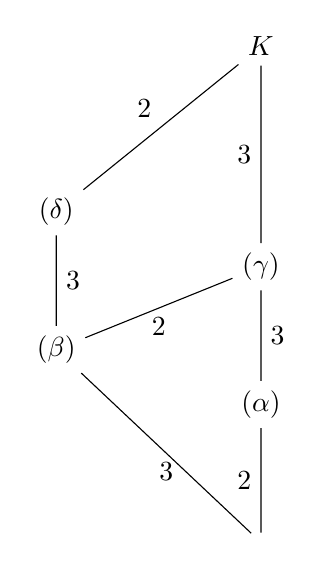
\begin{tikzpicture}[auto, xscale=.65, yscale=.35]
          \node(octic) at (8,23){$K$};
          \node(quart2) at (4,17){$\Q(\delta)$};
          \node(quart3) at (8,15){$\Q(\gamma)$};
          \node(quad1) at (4,12){$\Q(\beta)$};
          \node(quad2) at (8,10){$\Q(\alpha)$};
          \node(q) at (8,5){$\Q$};
          \draw (quad1) to node [below] {3} (q);
          \draw (quad2) to node [swap] {2} (q);
          \draw (quad1) to node [swap] {3} (quart2);
          \draw (quad1) to node [below] {2} (quart3);
          \draw (quad2) to node [swap] {3} (quart3);
          \draw (quart2) to node {2} (octic);
          \draw (quart3) to node {3} (octic);
        \end{tikzpicture}
        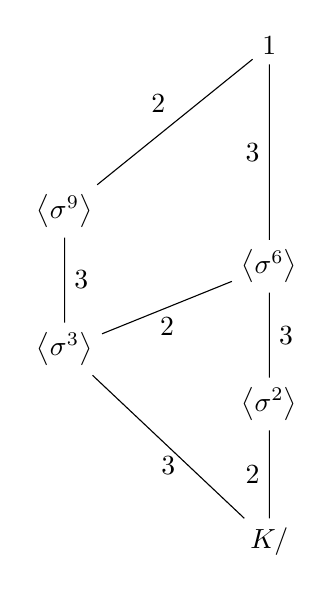
\begin{tikzpicture}[auto, xscale=.65, yscale=.35]
          \node(octic) at (8,23){$1$};
          \node(quart2) at (4,17){$\left<\sigma^9\right>$};
          \node(quart3) at (8,15){$\left<\sigma^6\right>$};
          \node(quad1) at (4,12){$\left<\sigma^3\right>$};
          \node(quad2) at (8,10){$\left<\sigma^2\right>$};
          \node(q) at (8,5){$\Gal{K/\Q}$};
          \draw (quad1) to node [below] {3} (q);
          \draw (quad2) to node [swap] {2} (q);
          \draw (quad1) to node [swap] {3} (quart2);
          \draw (quad1) to node [below] {2} (quart3);
          \draw (quad2) to node [swap] {3} (quart3);
          \draw (quart2) to node {2} (octic);
          \draw (quart3) to node {3} (octic);
        \end{tikzpicture}
      \end{center}
  \end{proof}
\end{thm}

\begin{thm}
  Prove that $\Q(\sqrt[3]{2})$ is not a subfield of any cyclotomic field over $\Q$.
  
  \begin{proof}
    Since the Galois group of a cyclotomic extension is abelian, all the subgroups are normal and so the subfields are Galois.
    Since $\Q(\sqrt[3]{2})$ is not Galois, it is not a subfield of any cyclotomic extension.
  \end{proof}
\end{thm}

\begin{thm}
  Let $p$ be an odd prime, and let $\zeta$ be a primitive $p^\text{th}$ root of unity.
  \begin{enumerate}[(a)]
  \item
    Show that $\Q(\zeta)$ has exactly one subfield, $K$, with $[K : \Q] = 2$.
  \item
    Show that $K$ is real if and only if $p \equiv 1 \pmod{4}$.
  \end{enumerate}
  
  \begin{proof}
    \begin{enumerate}[(a)]
    \item
      First observe that $\Gal{\Q(\zeta)/\Q} \cong (\Z/p\Z)^\times \cong \Z/(p-1)\Z$, which is cyclic.
      Since $p - 1 \equiv 0 \pmod{2}$, and cyclic groups have unique (up to isomorphism) subgroups of all orders dividing the order of the group, there exists a subgroup of order $(p-1)/2$, $H$.
      Then $[\Q(\zeta)^H : \Q] = [\Gal{\Q(\zeta)/\Q} : H] = 2$.
    \item
      Let $H \leq \Gal{\Q(\zeta)/\Q}$ be as above.
      First observe that because $K/\Q$ is Galois, it is also normal.
      Hence if $\sigma : \Q(\zeta) \hookrightarrow \C$ is complex conjugation, it follows from the normality of $\Q(\zeta)/\Q$ that $\sigma$ is the unique automorphism of order two in $\Gal{\Q(\zeta)/\Q}$.
      
      Observe that by the argument in the previous part, $H$ has a subgroup of order two if and only if two divides $(p-1)/2$.
      Moreover, two divides $(p-1)/2$ if and only if $p \equiv 1 \pmod{4}$.
      Since $\sigma$ is the unique element of order two, $\sigma \in H$ if and only if $p \equiv 1 \pmod{4}$.
      Hence complex conjugation fixes $K^H$ if and only if $p \equiv 1 \pmod{4}$.
      Therefore $K^H$ is real if and only if $p \equiv 1 \pmod{4}$.
    \end{enumerate}
  \end{proof}
\end{thm}
\end{document}
